\documentclass{article}

\usepackage{amsmath,amssymb}
\usepackage{mathrsfs}
\usepackage{braket}
\usepackage{graphicx}

\usepackage{textpos}
\usepackage{eso-pic}
\usepackage{tikz}
\usetikzlibrary{tikzmark}

\title{Connecting Particle and Field Mechanics}
\author{Anthony Mezzacappa}
\date{September 1 and 3, 2020}
% Typeset by Anjali Rathore
% Spring diagram by Wileam Phan

\begin{document}
\setlength{\parskip}{1em}
\maketitle

\noindent Consider we have a classical linear chain of equal masses connected by spring of equal spring constant. The springs can oscillate about there equilibrium position in one dimension. In equilibrium all masses are separated by an equal length. \par

$\kappa$ = value of the spring constant \par
$a$ = length between the masses in equilibrium\par
$m$ = mass of each of the sampled masses\par

\begin{figure}[h!]
    \centering
    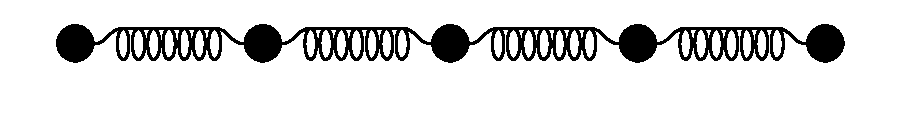
\includegraphics[width=\textwidth]{pics/04-linear-chain.pdf}
    \label{fig:l4-linear-chain}
\end{figure}

\noindent Define \par
$q_n(t) =$ displacement of each oscillator from its equilibrium position $\bar{q}_n \equiv na $ -- i.e., $x_n(t) = na+q_n(t)$

\noindent For simplicity, we will assume periodicity i.e.,
\begin{equation*}
    q_1(t) =q_{N+1}(t)
\end{equation*}
In the limit $N \rightarrow \infty$, this will not matter.

% Page 2

{%
\begin{textblock*}{2in}(0.88in,1.25in)%
\begin{minipage}[h!]{2in}
    \begin{equation*}
        \tikzmarknode{xdot}{\boxed{\dot{x}_n (t) = \dot{q}_n (t)}}
    \end{equation*}
\end{minipage}%
\end{textblock*}%
}

{%
\begin{textblock*}{3in}(2.7in,1.1in)%
\begin{minipage}[h!]{3in}
    \noindent it's only the difference in the displacements of the masses from their equilibrium position that \linebreak contributes to the potential energy
    \begin{align*}
        \big( x_{n+1} (t) - x_n (t) \big) - a &= ( n + 1 ) a + q_{n+1} (t) \\
        &\quad - n a - q_n (t) - a \\
        &= q_{n+1} (t) - q_n (t)
    \end{align*}
\end{minipage}%
\end{textblock*}%
}

\noindent The Lagrangian of this system is
\begin{align*}
    L &= T - V \\
    &= \frac{1}{2} m \sum_{n=1}^N \tikzmarknode{qdot}{\dot{q}_n^2} - \frac{1}{2} \kappa \sum_{n=1}^N \underbrace{ {(q_{n+1} - q_n)}^2 }
\end{align*}

\begin{tikzpicture}[overlay, remember picture]
    \draw[overlay,->] (xdot) -- (qdot.south);
\end{tikzpicture}

\noindent The Euler-Lagrangian EOM for each mass are
\begin{equation}
    \dfrac{ \partial L }{ \partial q_n} -  \dfrac{d}{ \mathrm{d} t} \left[\dfrac{ \partial L }{ \partial \dot {q}_n } \right] = 0
\end{equation}

\noindent $\dfrac{ \partial L }{ \partial q_n}$ :
\begin{align*}
    & -\tfrac{1}{2} \kappa \sum_{n=1}^N (q_{n+1} - q_n)^2 \\
    &= -\tfrac{1}{2} \kappa \left[(q_{2} - q_1)^2) + (q_{3} - q_2)^2 + (q_{4} - q_3)^2 + \dots \right. \\
    &\qquad \quad \left. + (q_{n} - q_{n-1})^2 + (q_{n+1} - q_n)^2 + \dots \right]
\end{align*}

\noindent Then
\begin{align*}
    \dfrac{ \partial L }{ \partial q_n} &= -\tfrac{1}{2} \kappa \left[ 2 (q_{n} - q_{n-1}) + 2 (q_{n+1} - q_n)(-1)  \right] \\
    &= - \kappa \left[2 q_{n} - q_{n-1} - q_{n+1}  \right] \\ \\
    \dfrac{ \partial L }{ \partial \dot q_n} &= m\dot{q}_n
\end{align*}

% Page 3

\noindent Then the Euler-Lagrange EOM read
\begin{equation*}
    \kappa \left[ q_{n+1} -2 q_{n} + q_{n-1} \right] - m \ddot{q}_n = 0
\end{equation*}

\noindent We can compute the canonically conjugate momentum, $p_n$,
\begin{equation*}
  p_n =  \dfrac{ \partial L }{ \partial \dot q_n}  = m \dot{q}_n \qquad \mathrm{(as ~ above)} 
\end{equation*}

\noindent The Hamiltonian now follows
\begin{align*}
    H &= \sum_{n=1}^N p_n \dot{q}_n - L \\
    &= \sum_{n=1}^N p_n \frac{p_n}{m} - \left[\frac{1}{2} m \sum_{n=1}^N {\left( \frac{p_n}{m} \right)}^2 - \tfrac{1}{2} \kappa \sum_{n=1}^N (q_{n+1} - q_n)^2 \right] \\
    &= \sum_{n=1}^N \left[ \frac{p_n^2}{m} - \frac{p_n^2}{2 m} + \tfrac{1}{2} \kappa (q_{n+1} - q_n)^2 \right] \\
    &= \sum_{n=1}^N \frac{p_n^2}{2 m} + \tfrac{1}{2} \kappa \sum_{n=1}^N (q_{n+1} - q_n)^2
\end{align*}

% Page 4

\noindent Finally, the Poisson Bracket is
\begin{align*}
    \left\lbrace q_n, p_{n'} \right\rbrace &= \sum_{n=1}^N \left( \dfrac{ \partial q_n }{ \partial q_k } \dfrac{ \partial p_{n'} }{ \partial p_k } - \dfrac{ \partial q_n }{ \partial p_k } \dfrac{ \partial p_{n'} }{ \partial q_k } \right) \\
    &= \sum_{n=1}^N \left( \delta_{nk} \delta_{n'k} \right) \\
    &= \delta_{nn} \delta_{n'n} \\
    &= \delta_{nn'}
\end{align*}
Now we need to solve the EOM for $q_n (t)$.

\noindent Let
\begin{equation*}
    q_n (t) = q_n e^{ i \omega t }
\end{equation*}

\noindent Then
\begin{equation*}
    -m q_n \left( i^2 \omega^2 e^{ i \omega t } \right) + \kappa \left( q_{n+1} - 2 q_n + q_{n-1} \right) e^{ i \omega t } = 0
\end{equation*}
or
\begin{equation*}
    \left( m \omega^2 - 2 \kappa \right) q_n + \kappa \left( q_{n+1} + q_{n-1} \right) = 0
\end{equation*}

\noindent This has the solution
\begin{equation*}
    q_n = \dfrac{ a_k }{ \sqrt{N} } e^{ i k n a }
\end{equation*}

% Page 5

\noindent Inserting
\begin{equation*}
    \left( m \omega^2 - 2 \kappa \right) \dfrac{1}{ \sqrt{N} } e^{ i k n a } + \kappa \dfrac{1}{ \sqrt{N} } e^{ i k n a } \left( e^{ i k a } + e^{ -i k a } \right) = 0
\end{equation*}

\noindent Then
\begin{equation*}
    \left( m \omega^2 - 2 \kappa \right) + 2 \kappa \cos{(ka)} = 0
\end{equation*}

\noindent This is the dispersion relation relating $\omega$ and $k$:
\begin{equation*}
    \omega^2 = \dfrac{1}{m} 2 \kappa \left( 1 - \cos{(ka)} \right) \qquad \Longrightarrow \qquad \dfrac{ 4 \kappa }{m} \sin^2{\left(\dfrac{ k a }{2}\right)} \Rightarrow \omega_\pm^2
\end{equation*}
or
\begin{align*}
    \omega_k &= \pm {\left[ \dfrac{ 2 \kappa }{m} \left( 1 - \cos{(ka)} \right) \right]}^\frac{1}{2} \\
    &= \pm 2 \sqrt{\dfrac{\kappa}{m}} \sin{\left( \dfrac{ka}{2} \right)} \quad \Longrightarrow \quad \omega_{-k} = \omega_{k} ~ \mathrm{where} ~ \omega_k \equiv 2 \sqrt{\dfrac{\kappa}{m}} \sin{\left( \dfrac{ka}{2} \right)}, k>0
\end{align*}

\noindent Now let
\begin{equation*}
    q_n (t) = q_n^* e^{ -i \omega t }
\end{equation*}

% Page 6

\noindent Then
\begin{equation*}
    -m q_n^* \left( i^2 \omega^2 e^{ -i \omega t } \right) + \kappa \left( q_{n+1}^* - 2 q_n^* + q_{n-1}^* \right) e^{ -i \omega t } = 0
\end{equation*}
or
\begin{equation*}
    \left( m \omega^2 - 2 \kappa \right) q_n^* + \kappa \left( q_{n+1}^* + q_{n-1}^* \right) = 0
\end{equation*}
which has the solution
\begin{equation*}
    q_n^* = \dfrac{ a_k^* }{ \sqrt{N} } e^{ -i k n a }
\end{equation*}

\noindent Inserting
\begin{equation*}
    \left( m \omega^2 - 2 \kappa \right) e^{ -i k n a } + \kappa e^{ -i k n a } \left( e^{ -i k a } + e^{ i k a } \right) = 0
\end{equation*}
or
\begin{equation*}
    \left( m \omega^2 - 2 \kappa \right) + 2 \kappa \cos{(ka)}
\end{equation*}
as before.

\noindent The general relation for $q_n (t)$ is then
\begin{equation*}
    q_n (t) = \dfrac{1}{\sqrt{N}} \sum_k \left( a_k e^{ i k n a } e^{ i \omega_k t } + a_k^* e^{ -i k n a } e^{ -i \omega_k t } \right)
\end{equation*}

% Page 7

\noindent To determine the values over which we sum $k$, recall that
\begin{equation*}
    q_1 (0) = q_{N+1} (0)
\end{equation*}
which means that
\begin{equation*}
    \sum_k \left( e^{ i k a } + e^{ -i k a } \right) = \sum_k \left( e^{ i k (N+1) a } + e^{ -i k (N+1) a } \right)
\end{equation*}

\noindent Then
\begin{align*}
    \sum_k \cos{(ka)} &= \sum_k \cos{[\underbrace{ k (N+1) a}_{ k N a + k a }]} \\
    &= \sum_k \left( \cos{(kNa)} \cos{(ka)} - \sin{(kNa)} \sin{(ka)} \right)
\end{align*}
which gives
\begin{align*}
    \cos{(kNa)} &= 1 \qquad \Longrightarrow \qquad k N a = 2 \pi l \qquad l = \pm 1, \pm 2, \dots \\
    \sin{(kNa}) &= 0 \qquad \qquad ( l = 0 ~ \mathrm{corresponds} ~ \mathrm{to} ~ \mathrm{a} ~ \mathrm{trivial} ~ \mathrm{solution} )
\end{align*}

\noindent Then
\begin{align*}
    q_n (t) &= \dfrac{1}{\sqrt{N}} \sum_l \left( a_l e^{ i \frac{2 \pi l n}{N}} e^{ i \omega_l t } + a_l^* e^{ -i \frac{2 \pi l n}{N}} e^{ -i \omega_l t } \right) \\
    &= \sum_l \left[ u_{n,l} a_l (t) + u_{n,l}^* a_l^* (t) \right]
\end{align*}
where
\begin{align*}
    u_{n,l} &= \dfrac{1}{\sqrt{N}} e^{ i \frac{ 2 \pi l n }{N} } \\
    a_l (t) &= a_l e^{ i \omega_l t }
\end{align*}

% Page 8

\noindent To determine the limits of $l$, note that the smallest wavelength that can fit on our chain is
\begin{equation*}
    \lambda_\mathrm{minimum} = 2a
\end{equation*}

\noindent Since
\begin{align*}
    \lambda &= \dfrac{2 \pi}{k} \\
    &= \dfrac{2 \pi}{\frac{2 \pi l}{ N a }} \\
    &= \dfrac{Na}{l}
\end{align*}
we have
\begin{align*}
    \lambda_\mathrm{min} &= \dfrac{N a}{l_\mathrm{max}} \\
    &= 2a
\end{align*}

\noindent Then
\begin{equation*}
    l_\mathrm{max} = \dfrac{N}{2}
\end{equation*}
and our sum over $l$ becomes
\begin{equation*}
    q_n (t) = \sum_{ l = -\frac{N}{2} }^{ +\frac{N}{2} }  \left[ a_l (t) u_{n,l} + a_l^* (t) u_{n,l}^* \right]
\end{equation*}

% Page 9

\noindent Now compute $p_n (t)$:
\begin{align*}
    p_n (t) &= m \dot{q}_n (t) \\
    &= m \sum_{ l = -\frac{N}{2} }^{ +\frac{N}{2} } i \omega_l \left[ a_l (t) u_{n,l} - a_l^* (t) u_{n,l}^* \right]
\end{align*}

\noindent Let's now compute the Hamiltonian:
\begin{equation*}
    H = \dfrac{1}{2m} \sum_{n=1}^{N} p_n^2 + \frac{1}{2} \kappa \sum_{n=1}^{N} {\left( q_{n+1} - q_n \right)}^2
\end{equation*}

\begin{align*}
    T &= \sum_{n=1}^{N} \dfrac{p_n^2}{2m} \\
    &= - \dfrac{m}{2} \sum_n \left\lbrace \left[ \omega_l \left( a_l (t) u_{n,l} - a_l^* (t) u_{n,l}^* \right) \right] \left[ \omega_{l'} \left( a_{l'} (t) u_{n,l'} - a_{l'}^* (t) u_{n,l'}^* \right) \right] \right\rbrace \\
    &= - \dfrac{m}{2} \sum_n \bigg\lbrace \sum_{l l'} \omega_l \omega_{l'} \Big( a_l (t) a_{l'} (t) u_{n,l} u_{n,l'} - a_l (t) a_{l'}^* (t) u_{n,l} u_{n,l'}^* \\
    & \hspace{1.4in} - a_l^* (t) a_{l'} (t) u_{n,l}^* u_{n,l'} + a_l (t)^* a_{l'}^* (t) u_{n,l}^* u_{n,l'}^* \Big) \bigg\rbrace 
\end{align*}

\noindent The orthogonality of the basis functions $u_{n,l}$ tells us that
\begin{align*}
    \sum_{n=1}^{N} u_{n,l'}^* u_{n,l} &= \delta_{l l'} \\
    \sum_{n=1}^{N} u_{n,l'} u_{n,l} &= \delta_{l,-l'} \\
    \sum_{n=1}^{N} u_{n,l'}^* u_{n,l}^* &= \delta_{l,-l'}
\end{align*}

% Page 10

\noindent Then
\begin{align*}
    T &= - \dfrac{m}{2} \sum_{l l'} \omega_l \omega_{l'} \Big( a_l (t) a_{l'} (t) \delta_{l,-l'} - a_l (t) a_{l'}^* (t) \delta_{l l'} \\
    & \hspace{1.1in} - a_l^* (t) a_{l'} (t) \delta_{l l'} + a_l (t)^* a_{l'}^* (t) \delta_{l,-l'} \Big) \\
    &= - \dfrac{m}{2} \sum_l \Big( \omega_l \underbrace{\omega_{-l}}_{=\omega_l} a_l (t) a_{-l} (t) - \omega_l^2 a_l (t) a_l^* (t) - \omega_l^2 a_l^* (t) a_l (t) + \omega_l \underbrace{\omega_{-l}}_{=\omega_l} a_l^* (t) a_{-l}^* (t) \Big) \\
    &= - \dfrac{m}{2} \sum_l \omega_l^2 \Big( a_l (t) a_{-l} (t) - a_l (t) a_l^* (t) - a_l^* (t) a_l (t) + a_l^* (t) a_{-l}^* (t) \Big) \\
    &= - \dfrac{m}{2} \sum_l \omega_l^2 \Big( a_l e^{ i \omega_l t } a_{-l} e^{ i \omega_{-l} t } - a_l e^{ i \omega_l t } a_l^* e^{ -i \omega_l t } \\
    & \hspace{0.9in} - a_l^* e^{ -i \omega_l t } a_l e^{ i \omega_l t } + a_l^* e^{ -i \omega_l t } a_{-l}^* e^{ -i \omega_{-l} t } \Big) \\
    &= - \dfrac{m}{2} \sum_l \omega_l^2 \Big( a_l a_{-l} e^{ 2i \omega_l t } - a_l a_l^* - a_l^* a_l + a_l^* a_{-l}^* e^{ -2i \omega_l t } \Big)
\end{align*}

% Pages 11-12

\noindent Now let's compute
\begingroup
\allowdisplaybreaks
\begin{align*}
    V &= \frac{1}{2} \kappa \sum_{n=1}^N {( q_{n+1} - q_n )}^2 \\
    &= \frac{1}{2} \kappa \sum_n {\Big\lbrace \sum_l \big[ \left( a_l (t) u_{n+1,l} + a_l^* (t) u_{n+1,l}^* \right) - \left( a_l (t) u_{n,l} + a_l^* (t) u_{n,l}^* \right) \big] \Big\rbrace}^2 \\
    %
    &= \frac{1}{2} \kappa \sum_n \sum_l \sum_{l'} \Big\lbrace \left( a_l (t) u_{n+1,l} + a_l^* (t) u_{n+1,l}^* \right) \left( a_{l'} (t) u_{n+1,l'} + a_{l'}^* (t) u_{n+1,l'}^* \right) \\
    & \hspace{1.1in} + \left( a_l (t) u_{n,l} + a_l^* (t) u_{n,l}^* \right) \left( a_{l'} (t) u_{n,l'} + a_{l'}^* (t) u_{n,l'}^* \right) \\
    & \hspace{1.1in} - \left( a_l (t) u_{n+1,l} + a_l^* (t) u_{n+1,l}^* \right)  \left( a_{l'} (t) u_{n,l'} + a_{l'}^* (t) u_{n,l'}^* \right) \\
    & \hspace{1.1in} - \left( a_l (t) u_{n,l} + a_l^* (t) u_{n,l}^* \right) \left( a_{l'} (t) u_{n+1,l'} + a_{l'}^* (t) u_{n+1,l'}^* \right) \Big\rbrace \\
    %
    &= \frac{1}{2} \kappa \sum_n \sum_l \sum_{l'} \Big\lbrace \left( a_l (t) e^{i \frac{2 \pi l}{N}} u_{n,l} + a_l^* (t) e^{-i \frac{2 \pi l}{N}} u_{n,l}^* \right) \left( a_{l'} (t) e^{i \frac{2 \pi l'}{N}} u_{n,l'} + a_{l'}^* (t) e^{-i \frac{2 \pi l'}{N}} u_{n,l'}^* \right) \\
    & \hspace{1.1in} + \left( a_l (t) u_{n,l} + a_l^* (t) u_{n,l}^* \right) \left( a_{l'} (t) u_{n,l'} + a_{l'}^* (t) u_{n,l'}^* \right) \\
    & \hspace{1.1in} - \left( a_l (t) e^{i \frac{2 \pi l}{N}} u_{n,l} + a_l^* (t) e^{-i \frac{2 \pi l}{N}} u_{n,l}^* \right)  \left( a_{l'} (t) u_{n,l'} + a_{l'}^* (t) u_{n,l'}^* \right) \\
    & \hspace{1.1in} - \left( a_l (t) u_{n,l} + a_l^* (t) u_{n,l}^* \right) \left( a_{l'} (t) e^{i \frac{2 \pi l'}{N}} u_{n,l'} + a_{l'}^* (t) e^{-i \frac{2 \pi l'}{N}} u_{n,l'}^* \right) \Big\rbrace \\
    %
    &= \frac{1}{2} \kappa \sum_l \sum_{l'} \Big\lbrace a_l (t) a_{l'} (t) e^{i \frac{2 \pi l}{N}} e^{i \frac{2 \pi l'}{N}} \delta_{l,-l'} + a_l (t) a_{l'}^* (t) e^{i \frac{2 \pi l}{N}} e^{-i \frac{2 \pi l'}{N}} \delta_{l,l'} \\
    & \hspace{0.9in} + a_l^* (t) a_{l'} (t) e^{-i \frac{2 \pi l}{N}} e^{i \frac{2 \pi l'}{N}} \delta_{l,l'} + a_l^* (t) a_{l'}^* e^{-i \frac{2 \pi l}{N}} e^{-i \frac{2 \pi l'}{N}} \delta_{l,-l'} \\
    & \hspace{0.9in} + a_l (t) a_{l'} (t) \delta_{l,-l'} + a_l (t) a_{l'}^* (t) \delta_{l,l'} + a_l^* (t) a_{l'} (t) \delta_{l,l'} + a_l^* (t) a_{l'}^* (t) \delta_{l,-l'} \\
    & \hspace{0.9in} - a_l (t) a_{l'} (t) e^{i \frac{2 \pi l}{N}} \delta_{l,-l'} - a_l (t) a_{l'}^* (t) e^{i \frac{2 \pi l}{N}} \delta_{l,l'} \\
    & \hspace{0.9in} - a_l^* (t) a_{l'} (t) e^{-i \frac{2 \pi l}{N}} \delta_{l,l'} - a_l^* (t) a_{l'}^* (t) e^{-i \frac{2 \pi l}{N}} \delta_{l,-l'} \\
    & \hspace{0.9in} - a_l (t) a_{l'} (t) e^{i \frac{2 \pi l'}{N}} \delta_{l,-l'} - a_l (t) a_{l'}^* (t) e^{-i \frac{2 \pi l'}{N}} \delta_{l,l'} \\
    & \hspace{0.9in} - a_l^* (t) a_{l'} (t) e^{i \frac{2 \pi l'}{N}} \delta_{l,l'} - a_l^* (t) a_{l'}^* (t) e^{-i \frac{2 \pi l'}{N}} \delta_{l,-l'} \Big\rbrace \\
    %
    &= \frac{1}{2} \kappa \sum_l \Big\lbrace a_l (t) a_{-l} (t) + a_l (t) a_l^* (t) + a_l^* (t) a_l (t) + a_l^* (t) a_{-l}^* (t) \\
    & \hspace{0.7in} + a_l (t) a_{-l} (t) + a_l (t) a_l^* (t) + a_l^* (t) a_l (t) + a_l^* (t) a_{-l}^* (t) \\
    & \hspace{0.7in} - a_l (t) a_{-l} (t) e^{i \frac{2 \pi l}{N}} - a_l (t) a_l^* (t) e^{i \frac{2 \pi l}{N}} \\
    & \hspace{0.7in} - a_l^* (t) a_l (t) e^{-i \frac{2 \pi l}{N}} - a_l^* (t) a_{-l}^* (t) e^{-i \frac{2 \pi l}{N}} \\
    & \hspace{0.7in} - a_l (t) a_{-l} (t) e^{-i \frac{2 \pi l}{N}} - a_l (t) a_l^* (t) e^{-i \frac{2 \pi l}{N}} \\
    & \hspace{0.7in} - a_l^* (t) a_l (t) e^{i \frac{2 \pi l}{N}} - a_l^* (t) a_{-l}^* (t) e^{i \frac{2 \pi l}{N}} \Big\rbrace \\
    \\
    &= \frac{1}{2} \kappa \sum_l \Big\lbrace a_l (t) a_{-l} (t) \left[ 2 - \left( e^{i \frac{2 \pi l}{N}} + e^{-i \frac{2 \pi l}{N}} \right) \right] \\
    & \hspace{0.7in} + a_l (t) a_l^* (t) \left[ 2 - \left( e^{i \frac{2 \pi l}{N}} + e^{-i \frac{2 \pi l}{N}} \right) \right] \\
    & \hspace{0.7in} + a_l^* (t) a_l (t) \left[ 2 - \left( e^{i \frac{2 \pi l}{N}} + e^{-i \frac{2 \pi l}{N}} \right) \right] \\
    & \hspace{0.7in} + a_l^* (t) a_{-l}^* (t) \left[ 2 - \left( e^{i \frac{2 \pi l}{N}} + e^{-i \frac{2 \pi l}{N}} \right) \right] \Big\rbrace \\
    %
    &= \kappa \sum_l \left( a_l (t) a_{-l} (t) + a_l (t) a_l^* (t) + a_l^* (t) a_l (t) + a_l^* (t) a_{-l}^* (t) \right) \big( \underbrace{ 1 - \cos{\left( \tfrac{ 2 \pi l }{N} \right)} }_{ 1 - \cos{(ka)} } \big)
\end{align*}
\endgroup

% Page 13

\noindent But
\begin{equation*}
    \dfrac{ m \omega_k^2 }{ 2 \kappa } =  1 - \cos{(ka)}
\end{equation*}

\noindent Then
\begin{equation*}
    V = \dfrac{m}{2} \sum_l \omega_l^2 \Big( a_l a_{-l} e^{ 2i \omega_l t } + a_l a_l^* + a_l^* a_l + a_l^* a_{-l}^* e^{ -2i \omega_l t } \Big)
\end{equation*}

\noindent Finally
\begin{align*}
    H &= T + V \\
    &= - \dfrac{m}{2} \sum_l \omega_l^2 \Big( a_l a_{-l} e^{ 2i \omega_l t } - a_l a_l^* - a_l^* a_l + a_l^* a_{-l}^* e^{ -2i \omega_l t } \Big) \\
    & \quad + \dfrac{m}{2} \sum_l \omega_l^2 \Big( a_l a_{-l} e^{ 2i \omega_l t } + a_l a_l^* + a_l^* a_l + a_l^* a_{-l}^* e^{ -2i \omega_l t } \Big) \\
    &= \sum_l m \omega_l^2 \Big( a_l^* a_l + a_l a_l^* \Big)
\end{align*}
But this is the Hamiltonian for a collection of \underline{uncoupled} oscillators, each one corresponding to a different normal mode of the system.

\noindent When we quantize this system, the quanta of the modes will correspond to the \underline{quasi-particles} known as \underline{phonons}.

\end{document}